\documentclass[a4paper,11pt]{article} %openright
\usepackage[a4paper, total={6in, 9in}]{geometry}
\usepackage[utf8]{inputenc}
\usepackage{amsfonts}
\usepackage{graphicx}

\title{
  Predictive Coding and Biologically Plausible Neural Networks \\
  \large{Bachelor Project}
}
\author{Anders Bredgaard Thuesen \\ s183926@student.dtu.dk}
\date{January 2022}

\begin{document}
\maketitle

\section*{Abstract}


\newpage

\tableofcontents

\newpage

\section{Introduction}
\subsection{Motivation}
In the recent years, deep learning has shown impressive results due to the availability of massive parallel compute and huge amounts of data. From the biological inspiration of the neuron to the perceptron where data inputs are weighted, summed together and thresholded, several new modern architectures, like recurrent, residual and transformer neural networks have pushed the limits and achieved state of the art results in speech recognition, computer vision and natural language understanding. Despite of these networks being originally inspired by the brain, the backpropagation (backprop) algorithm for learning the weights and deep learning in general has been criticized for being biologically implausible \cite{BengioLBL15}. This project will primarily be dealing with on of them: The weight transport problem which arises from the way backprop uses the connection weights in both the forward pass (inference) and the backwards parse (calculating the gradients), requiring that both forward and backward connections have symmetric weights and that information is able to flow backwards through the weights. \\
Besides having both philosophical as well scientific interest, studying the computational aspects of how the human brain processes sensory input might lead to great improvements in deep learning and artificial intelligence.

\subsection{Related work}
Several attempts has been made to make modern deep learning more biologically plausible. These can be divided into two types of categories. The first category consists of methods that try to optimize the inference on low-powered neuromorphic hardware such as the Intel Loihi or IBM TrueNorth chips, by converting existing neural network architectures into their spiking counterparts. The other category consists of methods that aim to make the learning phase biologically plausible by only relying on local weight updates in order to optimize for some objective. This is in alignment with the Hebbian learning theory from the neuroscience litterature which states that the synaptic plasticity is only dependent on the pre- and post-synaptic activity, possibly modulated through some global signaling mechasnism (ex. dopamine). One example hereof is the work by Bengio et al. on Continual Equilibrium Propagation \cite{EqProp}. 

\subsection{Research questions}
The project will address the following three research questions:
\begin{itemize}
  \item According to the current literature, what are the biological constraints of biological learning?
  \item To what extent can predictive coding be used to approximate backpropagation under the above mentioned biological constraints?
  \item In what ways can modern deep learning benefit from biological plausible learning algorithms?
\end{itemize}

\section{Classical deep learning}
\subsection{Dataset}
We define our dataset, $\mathcal{D} = \left\{(\mathbf{x}_i, \mathbf{y}_i)\right\}$ for $i = 1 \ldots N$ consisting of $N$ pairs of datapoints, $\mathbf{x}_i \in \mathbb{R}^k$ and $\mathbf{y}_i \in \mathbb{R}^l$ where $N$ is the size of the dataset. We notice, that both $\mathbf{x}_i$ and $\mathbf{y}_i$ can be vectors of possibly differently dimensions $k$ and $l$ respectively. Here $\mathbf{x}_i$ might represent eg. an image with its horizontal and channel axes flattened into a single one-dimensional vector, as we will encounter later when training on images of handwritten digits in the MNIST dataset \cite{mnist}. In the case of supervised learning, our objective is from $\mathbf{x}_i$ to predict the corresponding label, $\mathbf{y}_i$ which amounts to a single scalar number from 0 to 9 in the MNIST dataset. 
\begin{figure}[ht]
  \centering
  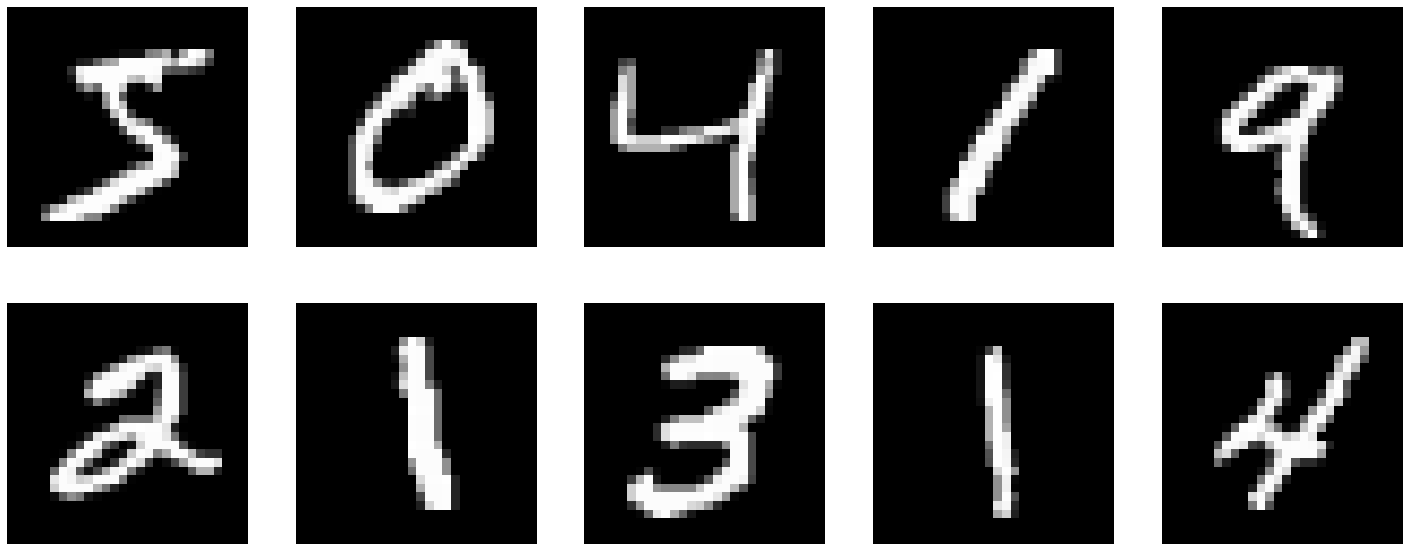
\includegraphics[width=280pt]{graphics/mnist.png}  
  \label{fig:MNIST}
  \caption{First 10 examples of the MNIST training dataset.}
\end{figure}
% TODO: Write more about mnist. How many training, test examples? What is the size of each image? Etc. Maybe also a little bit about fashion mnist. 


\subsection{Feedforward neural networks}
Feedforward neural networks (FNN) are considered the simplest kind of neural network where the connections between the nodes does not allow for any cycles or recurrent connections. Feedforward neural networks are divided into several layers, where input data from the first layer is "feed forward" through the so-called hidden layers to the final output layer of the network, considered the prediction of the network. FNNs are typically fully connected networks which entails that every node of the network is connected to every node in the previous layer. One special case of FNNs is that of when there are no hidden layers in the network and the input layer is linearly transformed to the output layer and "activated" through a softmax or sigmoid function, depending on the output of output nodes. In that case, the FNN will correspond to (multinomial) logistic regression. This correspondance incentivises the use of activation functions  after each linear transformation of the layers, as the network would otherwise not be able to describe non-linearities in the data. Historically, the sigmoid activation function $\sigma(z) = (1 + \exp(-z))^{-1}$ has been the go-to activation function, but recently the rectified linear unit, $\textrm{ReLU}(z) = \max(0, z)$, has become the de facto standard. \\
\\*
A feedforward neural network with $L-2$ hidden layers is parametarized by the weight matrices $\mathbf{W}^{(l)} \in \mathbb{R}^{m \times n}$ and biases $\mathbf{b}^{(l)} \in  \mathbb{R}^{m}$ for $l = 2 \ldots L$ where $n$ is the input dimension of the layer and $m$ the output dimension. A feedforward pass from layer $l-1$ to layer $l$ is given by $\mathbf{a}^{(l)} = \sigma(\mathbf{z}^{l})$ where $\mathbf{z}^{(l)} = \mathbf{W}^{(l)} \mathbf{a}^{(l-1)} + \mathbf{b}^{(l)}$ and $\sigma$ is the chosen activation function. By letting the initial activation $\mathbf{a}^{(1)} = \mathbf{x}_i$ one can consider the final activation of the network the prediction of the network $\mathbf{\hat{y}}_i = \mathbf{a}^{(L)}$. \\
\\*
We initialize the weight matrices using Kaiming He initialization, where the entries of the matrix $W^{(l)}_{ij}$ are drawn from a normal distribution with zero mean and $\sqrt{2/n}$ standard deviation as this will help reduce vanishing and exploding gradient problem by keeping the variance in each layer equal when using ReLU activation. \cite{he2015delving}


\subsection{Back-propagation}
The working horse of allmost all modern deep learning models is the back-propagation (aka. backprop) algorithm first popularized for training neural networks by Rumelhart, Hinton \& Williams in 1986 \cite{rumelhart1986learning}. The algorithms solves what is referred to as the \textit{credit-assignment problem}. When learning the parameters of an artificial neural network we would like to know how changing a weight in the network contributes to the total loss, in order to change it in the direction that minimizes the loss. One naive way to do this would be simply to adjust a single random weight slightly, evaluate the new neural network on the dataset and observe the effect on the model loss. If the change leads to a decrease in loss, keep the change, otherwise repeat from the beginning. This would however be very computationally expensive, since the network would have to be evaluated on the entire dataset for each weight in the network. Fortunately, the backprop algorithm achieves this much more efficiently. \\
\\*
Back-propagation frames learning the parameters of the network or weights and biases as an optimization problem for some loss function, $\mathcal{L}(\hat{\mathbf{y}}, \mathbf{y})$, which measures the difference between the predicted output of the network, $\hat{\mathbf{y}}$, and the true output, $\mathbf{y}$. The weights and biases are then changed in order to minimize this difference. Examples of loss functions are squared error $\sum \frac{1}{2}(\hat{\mathbf{y}} - \mathbf{y})^2$, typically used for regression and categorical cross entropy $-\sum \mathbf{y} \cdot \log(\hat{\mathbf{y}})$ for classification. \\
\\*


\begin{equation}
  \Delta W^{(L)} = -\alpha \frac{\partial \mathcal{L}}{\partial W^{(L)}}
\end{equation}
%By first considering the output layer of the network, 

\section{Biologically plausible deep learning}
\subsection{Biological constraints}
Write something about biological constraints here.
\subsection{Spiking Neural Networks}
Define spiking neural networks here. Why are they cool?
\subsubsection{LIF Neuron model}
What are LIF neurons? What are their dynamics?
\subsubsection{ANN to SNN conversion}
How do we convert an ANN to a SNN and run the stuff live?
\subsection{Predictive Coding and Z-IL}
What is predictive coding? Mention Rao and Ballard. How can they calculate gradients? 
\subsubsection{Equivalence to back-prop}

\subsubsection{Variational free energy}
\subsection{Variational Inference}
\subsection{Energy Based Models}

\section{Results}

\section{Discussion}

\section{Conclusion}

\newpage
\bibliographystyle{plain}
\bibliography{refs}


\end{document}
